\documentclass{standalone}

\usepackage{tikz}
\usepackage{pgfplots}
\usepgfplotslibrary{statistics}
\usetikzlibrary{pgfplots.statistics}
\usepackage{etoolbox}

\newtoggle{label}
\togglefalse{label}

\pgfplotsset{compat=1.12}

\begin{document}
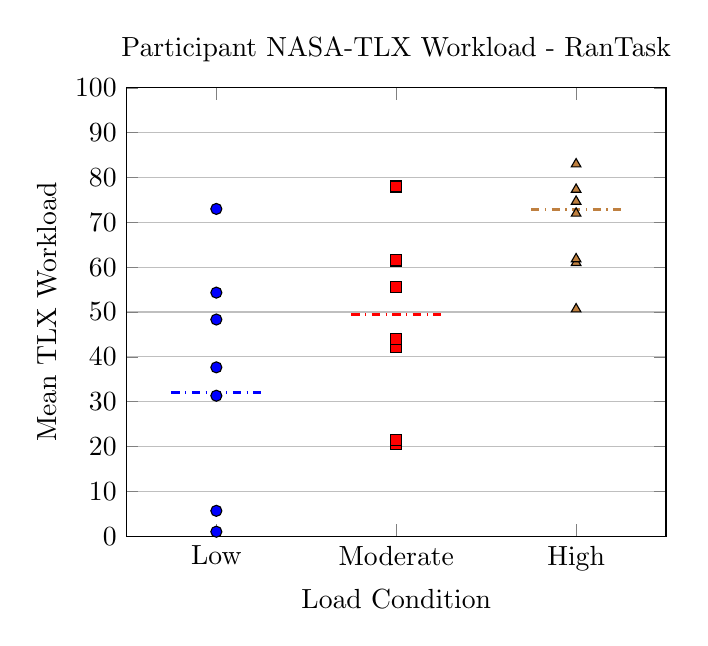
\begin{tikzpicture}
\begin{axis}[
	ymajorgrids,
	scatter/classes= {
		a={mark=*, fill=blue, draw=black},
		b={mark=square*, fill=red, draw=black},
		c={mark=triangle*, fill=brown, draw=black},
		d={mark=diamond*, fill=gray, draw=black}
	},
	ymin=0,
	ymax=100,
	xmin = .5, 
	xmax=3.5,
	ytick={0,10,...,100},
	xtick={1,2,3},
	xticklabel style={align=center},
	xticklabels={Low, Moderate, High},
	title=Participant NASA-TLX Workload - RanTask, 
	ylabel=Mean TLX Workload,
	xlabel=Load Condition]

	% Low
	\addplot+[ scatter,
			only marks,
			scatter src=explicit symbolic]
	coordinates {
			(1, 5.66)	[a]
			(1, 54.33)	[a]
			(1, 1.00)	[a]
			(1, 37.66)	[a]
			(1, 73.00)	[a]
			(1, 48.33)	[a]
			(1, 31.33)	[a]
};
\addplot+[ mark=None, dashdotted, blue, line width = 1pt ] 
	coordinates {
		(0.75, 32.02)
		(1.25, 32.02)
};

	% Moderate
	\addplot+[ scatter,
			only marks,
			scatter src=explicit symbolic]
	coordinates {
			(2, 20.66)	[b]
			(2, 42.16)	[b]
			(2, 21.50)	[b]
			(2, 44.00)	[b]
			(2, 78.00)	[b]
			(2, 55.66)	[b]
			(2, 61.50)	[b]
};
\addplot+[ mark=None, dashdotted, red, line width = 1pt ] 
	coordinates {
		(1.75, 49.5)
		(2.25, 49.5)
};

	% High
	\addplot+[ scatter,
			only marks,
			scatter src=explicit symbolic]
	coordinates {
			(3, 83.00)	[c]
			(3, 61.00)	[c]
			(3, 50.66)	[c]
			(3, 61.83)	[c]
			(3, 72.00)	[c]
			(3, 74.66)	[c]
			(3, 77.33)	[c]
};
\addplot+[ mark=None, dashdotted, brown, line width = 1pt ] 
	coordinates {
		(2.75, 72.92)
		(3.25, 72.92)
};


\end{axis}
\end{tikzpicture}

\end{document}
















